\documentclass[10pt, a4paper]{article}
\usepackage[left=2.00cm, right=2.00cm, top=2.00cm, bottom=2.00cm]{geometry}
\usepackage{supertabular}
\usepackage{graphicx}
\usepackage{float}
\usepackage[fontset=windows]{ctex}
\usepackage{amsmath,amssymb,amsthm}
\usepackage{unicode-math}
\usepackage{verbatim}
\usepackage{multirow}
\usepackage{pifont}
\usepackage{caption}
\usepackage{diagbox}
\usepackage{listings}
\usepackage{algorithm}  
\usepackage{algpseudocode}
\usepackage{booktabs}   
\usepackage{underscore}
\usepackage{xcolor}
\lstset{
  %行号
  numbers=left,
  %背景框
  frame=single,
  rulecolor=\color[rgb]{0.8,0.8,0.8},         % 设置代码框颜色
  breaklines,                                 % 自动将长的代码行换行排版
  extendedchars=false,                        % 解决代码跨页时,章节标题,页眉等汉字不显示的问题
  %背景色
  %backgroundcolor=\color[rgb]{1,1,0.76},
  backgroundcolor=\color[RGB]{245,245,244},
  %样式
  keywordstyle=\bf\color{blue},
  identifierstyle=\bf,
  numberstyle=\color[RGB]{0,192,192},
  commentstyle=\it\color[RGB]{0,96,96},
  stringstyle=\rmfamily\slshape\color[RGB]{128,0,0},
  %显示空格
  showstringspaces=false
}
% \begin{figure}[H]
%     \centering
%     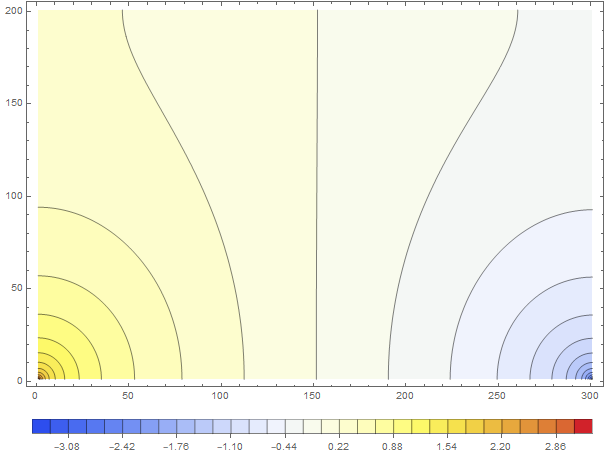
\includegraphics[width=0.4\textwidth]{Q1(1).png}
%     \caption{Q1(1)}\label{fig:Q1(1)}
% \end{figure}
\setcounter{secnumdepth}{4}
\setcounter{tocdepth}{4}
\newcommand{\whiteding}[1]{\ding{\numexpr171+#1\relax}}
\newcommand\vbf{\symbfit}
\newtheorem{definition}{\hspace{2em}定义}
\newtheorem{theorem}{\hspace{2em}定理}
\renewcommand{\algorithmicrequire}{\textbf{Input:}}  % Use Input in the format of Algorithm  
\renewcommand{\algorithmicensure}{\textbf{Output:}} % Use Output in the format of Algorithm  

\title{\heiti 大作业7\phantom{   }第二类永动机}
\author{ 张钰坤 \\  2000011314 \\(C语言实现)}
\date{2022年6月18日}

\begin{document}
    \maketitle
    \tableofcontents
    \newpage

    \section{第一问}
    漏洞:A,B两个黑体一定是有限大小的,而并非一个理想点。

    解释:题干论述中假设了A,B是两个点黑体,这样从几何上而言,从A发出的光才会全部达到B。现实中并不存在体积无穷小的点状黑体,A,B一定具有一个有限大的尺寸,于是,从A发出的光线就不一定能全部到达B了,比如下图中这种从A射向小椭球拱顶的光线根据对称性就一定都会返回A.

    \begin{figure}[H]
        \centering
        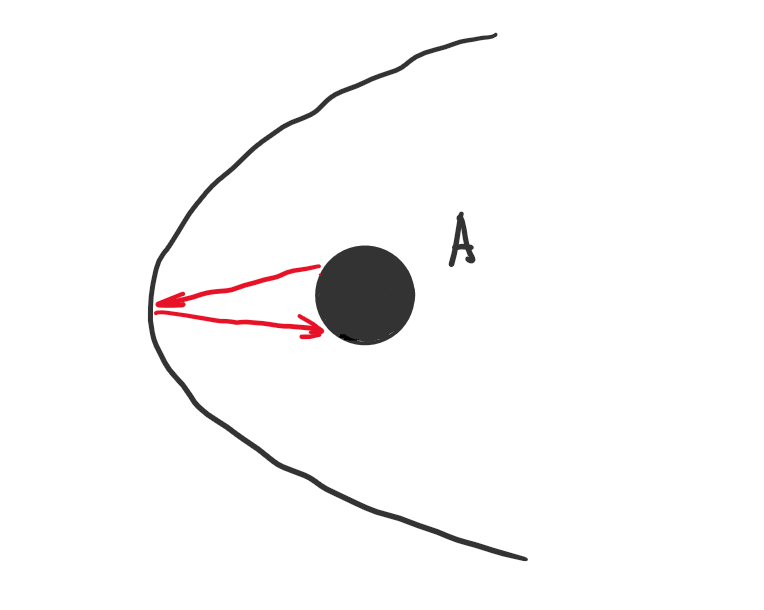
\includegraphics[width=0.4\textwidth]{q1特殊光线.png}
        \caption{q1特殊光线}\label{fig:q1特殊光线}
    \end{figure}

    于是,从A,B发出的光其实都有一部分返回、有一部分到达对方,于是就不能论证光线谁向谁流动的多,于是就不能判断有一个净能量流动。因此,考虑有限大黑体源,题干中的论述不一定成立。但具体成不成立,下面的数值模拟实验会说明:对于任意有限大黑体源,这类永动机都是失败的,热力学第二定律依然成立。

    \section{第2-5问解题思路}

    第2问需要计算任意给定一条初始光线,计算光线被吸收前的径迹。第3-5问是在不断缩小黑体A,B的尺寸,进行统计试验,以验证这类永动机的合理性。第3-5问比第2问只是多一个随机抽样的方法,剩下的只不过是将第二问重复很多很多次。所以,关键还是第二问的实现。
    
    第二问的实现分为两个部分。第一个部分是初始光线该如何描述,第二部分是光线的传播和演化。下面将分别介绍。

    \subsection{描述初始光线}

    如图所示,任意一条光线从球面上一点射出,设球的半径为R,不妨先以球心为原点。

    \begin{figure}[H]
        \centering
        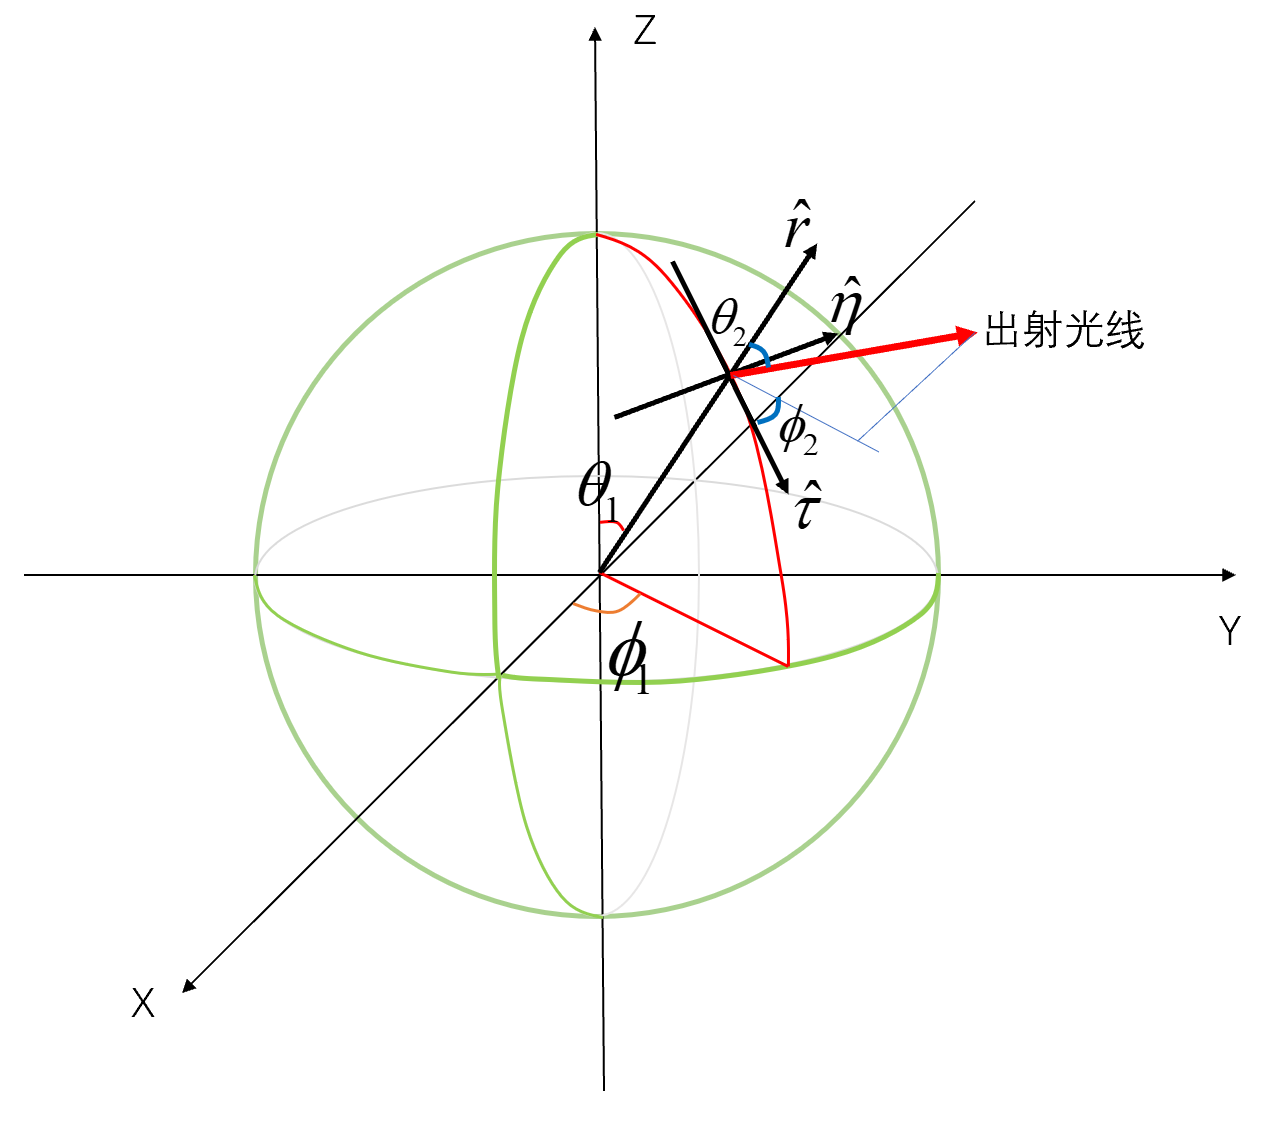
\includegraphics[width=0.6\textwidth]{出射光线坐标表示示意图.png}
        \caption{出射光线坐标表示示意图}\label{fig:出射光线坐标表示示意图}
    \end{figure}

    出射光线可以用出射点r和出射方向n来描述。而这两个向量可以由图中四个角度$(\theta_1,\phi1,\theta2,\phi2)$唯一确定。
    
    出射坐标表示为\[\vbf{r}=R(\sin\theta_1\cos\phi_1,\sin\theta_1\sin\phi_1,\cos\theta_1)\]

    合成上球心坐标就是真实出射坐标了,即

    \[\vbf{r}=\vbf{R_{\text{球心}}}+R(\sin\theta_1\cos\phi_1,\sin\theta_1\sin\phi_1,\cos\theta_1)\]

    同时可以得到

    \[\hat{r}= (\sin\theta_1\cos\phi_1,\sin\theta_1\sin\phi_1,\cos\theta_1)\]

    设$\hat{\tau}$与$\hat{r}$和z轴在同一平面,且$\hat{\tau}$与$\hat{r}$垂直,于是得到
    
    \[\hat{\tau}=(\cos\theta_1\cos\phi_1,\cos\theta_1\sin\phi_1,-\sin\theta_1)\]

    于是令$\hat{\eta}=\hat{r}\times\hat{\tau}$得到

    \[\hat{\eta}=(-\sin\phi_1,\cos\phi_1,0)\]

    设$\theta_2$为出射光线与$\hat{r}$的夹角,$\phi_2$为出射光线在$\hat{\tau},\hat\eta$平面内投影与$\hat\tau$的夹角。

    那么出射光线的方向向量为

    \[\vbf{n}=\sin\theta_2\cos\phi_2\hat\tau+\sin\theta_2\sin\phi_2\hat\eta+\cos\theta_2\hat r\]

    综上所述,描述出射光线的r和n可以写为

    \begin{align}
        \vbf{r}&=\vbf{R_{\text{球心}}}+R(\sin\theta_1\cos\phi_1,\sin\theta_1\sin\phi_1,\cos\theta_1)\\
        \vbf{n}&=\sin\theta_2\cos\phi_2
        \begin{pmatrix}
            \cos\theta_1\cos\phi_1\\\cos\theta_1\sin\phi_1\\-\sin\theta_1
        \end{pmatrix}
        +\sin\theta_2\sin\phi_2
        \begin{pmatrix}
            -\sin\phi_1\\\cos\phi_1\\0
        \end{pmatrix}
        +\cos\theta_2
        \begin{pmatrix}
            \sin\theta_1\cos\phi_1\\\sin\theta_1\sin\phi_1\\\cos\theta_1
        \end{pmatrix}
    \end{align}

    \subsection{光线的传播和演化}
    光线的传播可以分解为许多元过程:光线从一个接触点行进到下一个接触点。光线经过一个接触点之后,如果还要继续演化(即发生反射),那么反射后光线相当于从反射点射出一条方向固定的光线,直到碰到离它最近的物体为止。如果碰到黑体,那么光线被吸收,演化结束;如果碰到反射体,光线被反射,可以计算反射后的方向向量,于是开始了下一次元过程。

    所以,我们只需要编写一个程序来实现这个元过程,通过元过程的循环,就实现了光线的传播。这个元过程的功能是这样的,已知一个初始光线发射点坐标$\vbf{r_0}$和初始发射方向$\vbf{n_0}$,求出下一次与反射体或黑体接触时的坐标,如果与黑体接触,要判断是与A还是B接触的,如果与反射体接触,要计算发射后的新的方向向量。

    我们用函数来实现这个元过程,因为这个函数要返回很多信息,我们需要先把这些信息封装为一个结构体,如下

    \begin{lstlisting}[language=C]
        typedef struct transition{
            int situation;
            char absorb;
            vector* r;
            vector* n;
        }transition;
    \end{lstlisting}

    其中transition::situation只能取0,1,2。其中0表示计算遇到错误,1表示光线在当前元过程结束后被吸收,2表示光线在当前元过程结束后被反射。

    transition::absorb只能取'A','B'。其中'A'表示光线被黑体A吸收,'B'表示光线被黑体B吸收。

    transition::r表示光线下一个接触点的坐标。

    transition::n表示光线在下一个接触点被反射时反射光线的方向向量。

    值得注意的是,transition::situation=0时,其他变量都没有意义,当前计算有错;transition::situation=1时,只有transition::absorb和transition::r有意义;transition::situation=2时,只有transition::r和transition::n有意义。

    于是,我们的新编函数就可以返回一个指向transition的指针,就可以把所有信息传递出来。

    \begin{lstlisting}[language=C]
        transition* oneTransition(vector *r0,vector *n0);
    \end{lstlisting}

    这个函数内部的关键在于如何判断光线与哪个物体相交。光线一共与5个物体可能相交,我们将他们编号,如下图所示

    \begin{figure}[H]
        \centering
        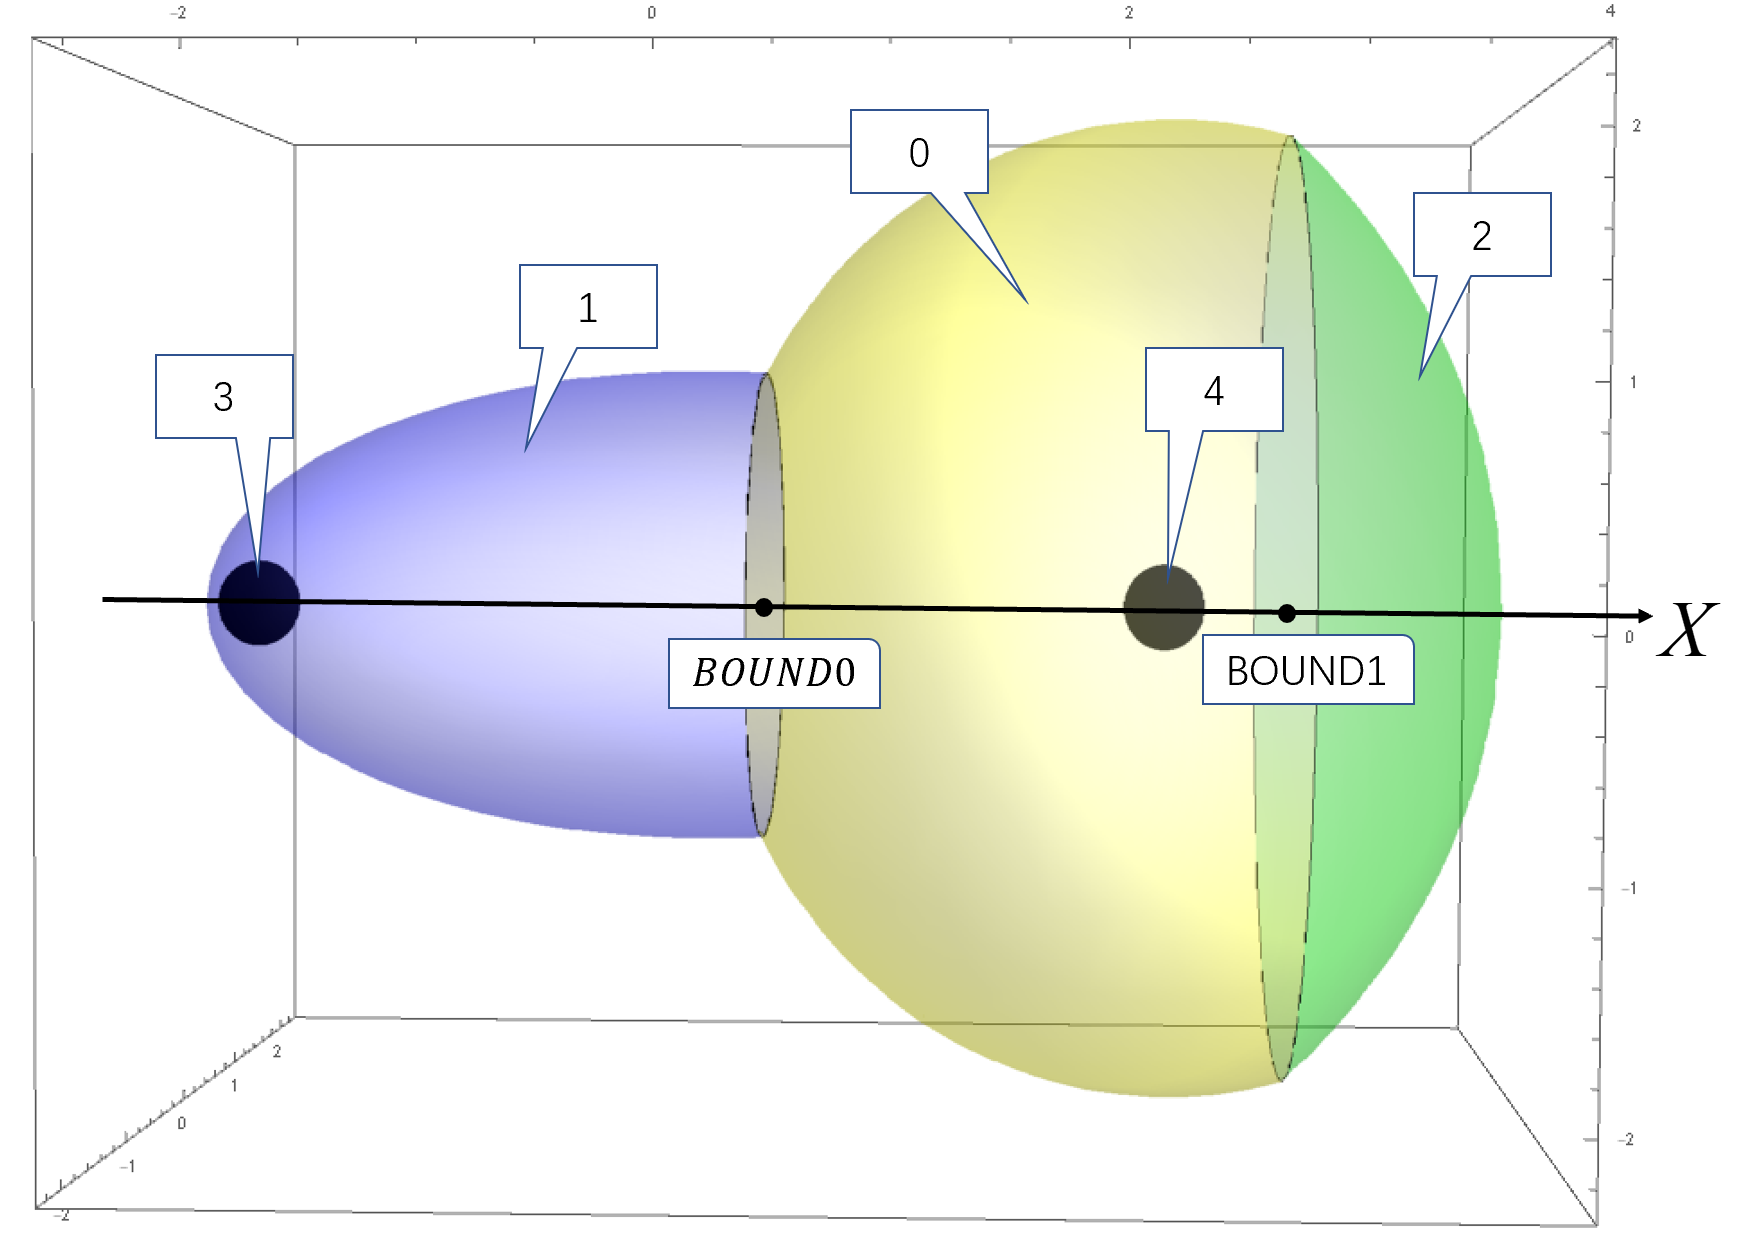
\includegraphics[width=0.6\textwidth]{物体编号示意图.png}
        \caption{物体编号示意图}\label{fig:物体编号示意图}
    \end{figure}

    设大小椭球共焦半焦距为c,小椭球半长轴、半短轴为$a_1,b_1$,大椭球半长轴半短轴$a_2,b_2$,黑体A,B的半径$RA,RB$.
    \begin{align*}
        0:&(x-c)^2+y^2+z^2=c^2,BOUND0<x<BOUND1\\
        1:&\frac{x^2}{a_1^2}+\frac{y^2+z^2}{b_1^2}=1,x<BOUND0\\
        2:&\frac{x^2}{a_2^2}+\frac{y^2+z^2}{b_1^2}=1,x>BOUND1\\
        3:&(x+c)^2+y^2+z^2=RA^2\\
        4:&(x-c)^2+y^2+z^2=RB^2
    \end{align*}

    由于已知光线的初始坐标和发射方向$\vbf{r_0},\vbf{n_0}$,光线可以写成参数方程

    \begin{align}\label{aln:光线参数方程}
        \vbf{r}=\vbf{r_0}+\vbf{n_0}t
    \end{align}

    把参数方程\ref{aln:光线参数方程}代入物体方程中,由于物体方程都是二次方程,我们将得到一个关于时间t的二次方程,以1号物体为例,记
    $\vbf{r_0}=(x_0,y_0,z_0),\vbf{n_0}=(n_{10},n_{20},n_{30})$

    \begin{align*}
        &\frac{(x_0+n_{10}t)^2}{a_1^2}+\frac{(y_0+n_{20}t)^2+(z_0+n_{30}t)^2}{b_1^2}=1\\
        \implies & A t^2+Bt+C=0\\
        where\text{ }& A=\frac{n_{10}^2}{a_1^2}+\frac{n_{20}^2+n_{30}^2}{b_1^2}\\
        &B=\frac{2n_{10}x_0}{a_1^2}+\frac{2n_{20}y_0+2n_{30}z_0}{b_1^2}\\
        &C=\frac{x_{0}^2}{a_1^2}+\frac{y_{0}^2+z_{0}^2}{b_1^2}-1
    \end{align*}

    每个联立所得到的二次方程都可以得到光线与对应物体的可能的位置关系。当二次方程没有正根的时候,表示光线不可能打到这个物体上,当二次方程有正根的时候,光线可能打到这个物体上。需要注意的是,由于$\vbf{r_0}$有可能是某个物体上的点,因此t在0附近可能会有一个根,但是这个跟不满足条件,当作没有它处理,所以正根的判断条件不应是t>0,而是t大于一个比较小的数,比如$t>10^{-7}$。还要特别注意的是,有些方程有定义域的限制,如果这个正根使得交点不在定义域内,这个正根也是应该舍去的。

    于是,五个联立所得的关于时间的二次方程将得到至多五个相交时刻(有的方程得不到相交时刻),在那些合理的相交时刻中取最小的那个,就是真实的光线遇到物体的时刻。接下来根据这个物体的编号,判断是被反射还是吸收,可以进行相应的计算。

    (transition*)oneTransition(vector*,vector*)函数具体实现见源代码文件。

    \subsection{抽样方法}

    对于第3-5问需要对生成随机的初始光线,由于每条初始光线都可由$(\theta_1,\phi_1,\theta_2,\phi_2)$唯一确定,因此需要对这四个参数进行抽样。这里采用直接抽样方法。

    设黑体单位面积发出的光线是定值,根据$dS\varpropto \sin\theta_1 d\theta_1 d\phi_1$,于是

    \begin{align*}
        \rho(\theta_1)&= \frac{1}{2}\sin\theta_1(\theta_1\in[0,\pi]) & \rho(\phi_1)=\frac{1}{2\pi}(\phi_1\in[0,2\pi))
    \end{align*}

    设黑体是朗伯辐射体,单位立体角发出的光线正比于$\cos\theta_2$,于是令
    \begin{align*}
        \rho(\theta_2)&=\sin\theta_2\cos\theta_2(\theta_2\in[0,\pi/2])&\rho(\phi_2)=\frac{1}{2\pi}(\phi_2\in[0,2\pi))
    \end{align*}

    则根据直接抽样方法,设$\xi $是某一0-1区间上的随机数,那么
    
    \begin{align*}
        \theta_1&=\arccos(1-2\xi)\\
        \phi_1&=2\pi\xi\\
        \theta_2&=\frac{1}{2}\arccos(1-2\xi)\\
        \phi_2&=2\pi\xi
    \end{align*}

    \subsection{一些几何运算}

    \subsubsection{计算反射体参数}

    由于旋转对称性,可以把三维问题当作二维问题计算,已知小椭圆半长轴$a_1=2.5$,偏心率$e=0.9$,大圆半径与小椭圆半焦距相同,为c。

    联立小椭圆和大圆得到交点$(x_0,y_0)$,
    \begin{align*}
        &\frac{x^2}{a_1^2}+\frac{y^2}{(a_1e)^2}=1\\
        &(x-c)^2+y^2=c^2
    \end{align*}

    解得
    \begin{align*}
        x_0&=a_1(\frac{1}{e}-1)(\text{舍去大于}a_1\text{的根}),y_0=a_1\sqrt{(1-e^2)(\frac{2}{e}-\frac{1}{e^2})}
    \end{align*}

    连接小椭圆左焦点和$(x_0,y_0)$作直线,交大圆于另一点$(x_1,y_1)$

    \begin{align*}
        &(x-c)^2+y^2=c^2\\
        &y=k_0(x+c),k_0=\frac{y_0}{x_0+c}
    \end{align*}

    解得

    \begin{align*}
        x_1&=2c\frac{1-k_0^2}{1+k_0^2}-x_0\\
        y_1&=k_0(x_1+c)
    \end{align*}

    由于大椭圆$\frac{x^2}{a_2^2}+\frac{y^2}{a_2^2-c^2}=1$一定过$(x_1,y_1)$,代入可解出$a_2$.

    解得

    \begin{align*}
        &(x_0,y_0)=(\frac{5}{18},\frac{\sqrt{95}}{9})\\
        &(x_1,y_1)=(\frac{342}{121},\frac{27\sqrt{95}}{121})\\
        &a_2=\frac{171}{44}
    \end{align*}

    \subsubsection{反射后的方向向量}

    \begin{figure}[H]
        \centering
        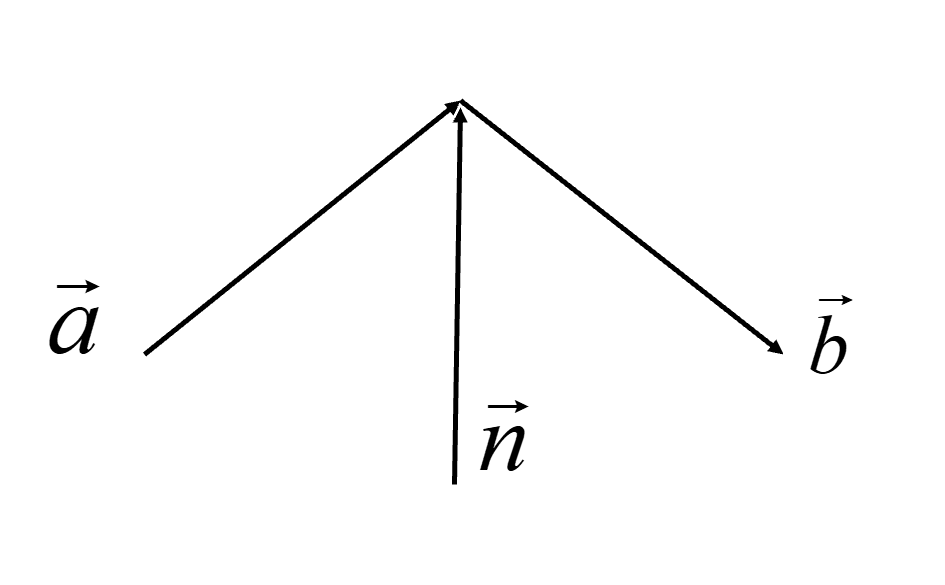
\includegraphics[width=0.3\textwidth]{反射向量计算示意图.png}
        \caption{反射向量计算示意图}\label{fig:反射向量计算示意图}
    \end{figure}

    如图,反射向量由$\vbf{b}=\vbf{a}-2(\vbf{a}\cdot\vbf{n})\vbf{n}$,其中$\vbf{n}$已经归一化。

    而对于曲面$F(x,y,z)=0$,(x,y,z)处法向量为$\nabla F(x,y,z)$给出。

    \section{代码实现导引和结果展示}

    \subsection{第二问}

    本题第二问源代码见code文件夹"plotTransition.c",不用手调参数除非更改初始条件,程序将在data/q2文件夹自动打出"q2_plotX.txt"(X=1,2,3,4,5,6)六个文件,可用plot中mathematica文件"plot_q2.nb"读取数据画出图像。注意mathematica中输入的是\textbf{绝对路径},需要手动更改路径。

    六个初始条件在代码注释中已经写明。

    将六幅光路图展示如下

    \begin{figure}[H]
        \centering
        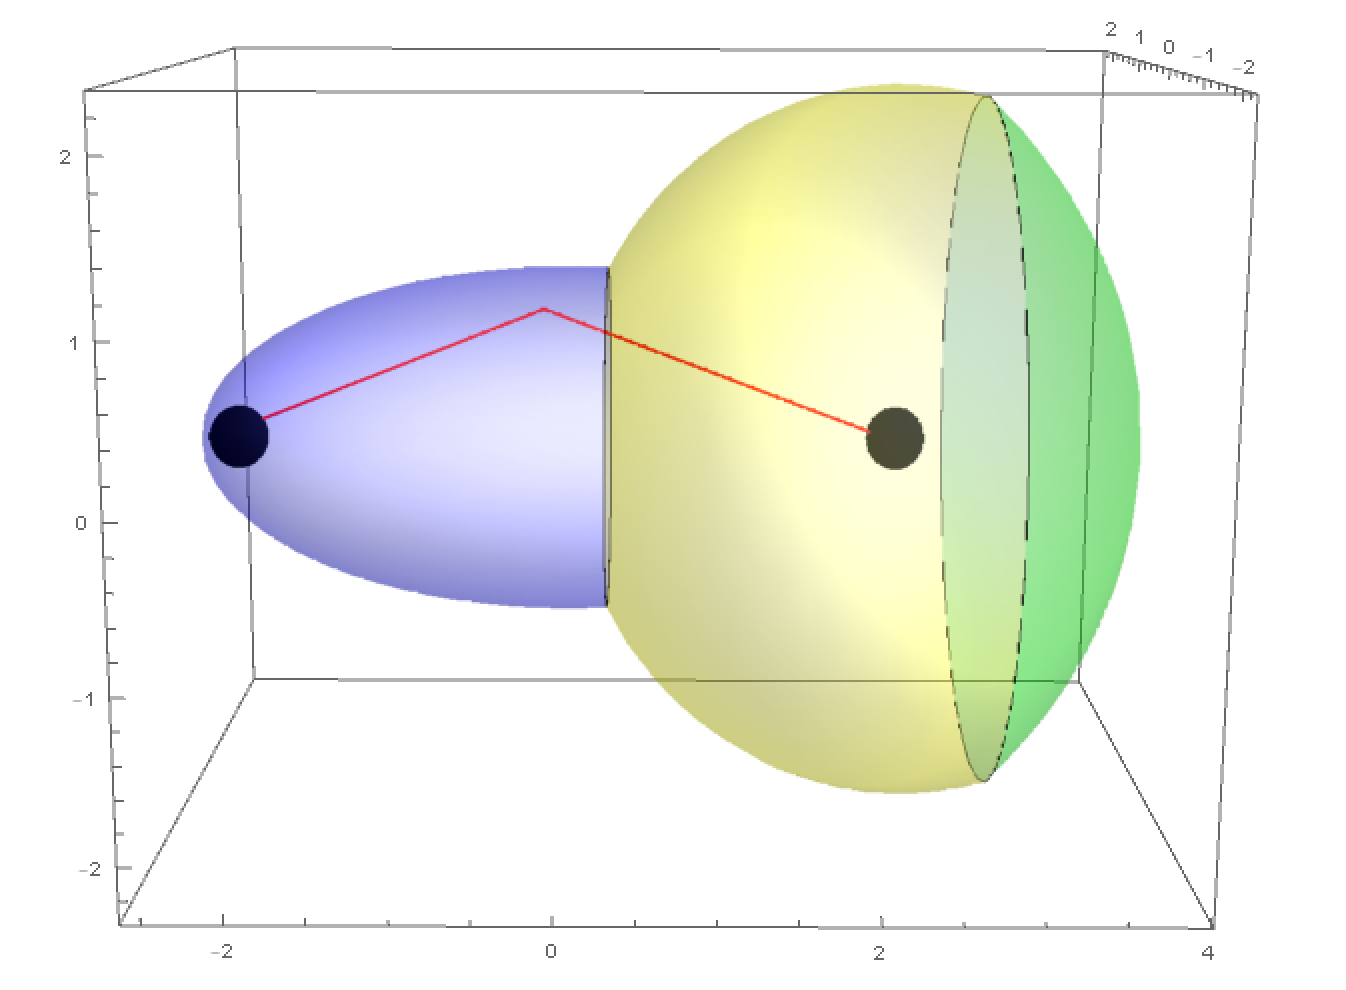
\includegraphics[width=0.6\textwidth]{q2_plot1.png}
        \caption{第二问plot1}\label{fig:第二问plot1}
    \end{figure}

    \begin{figure}[H]
        \centering
        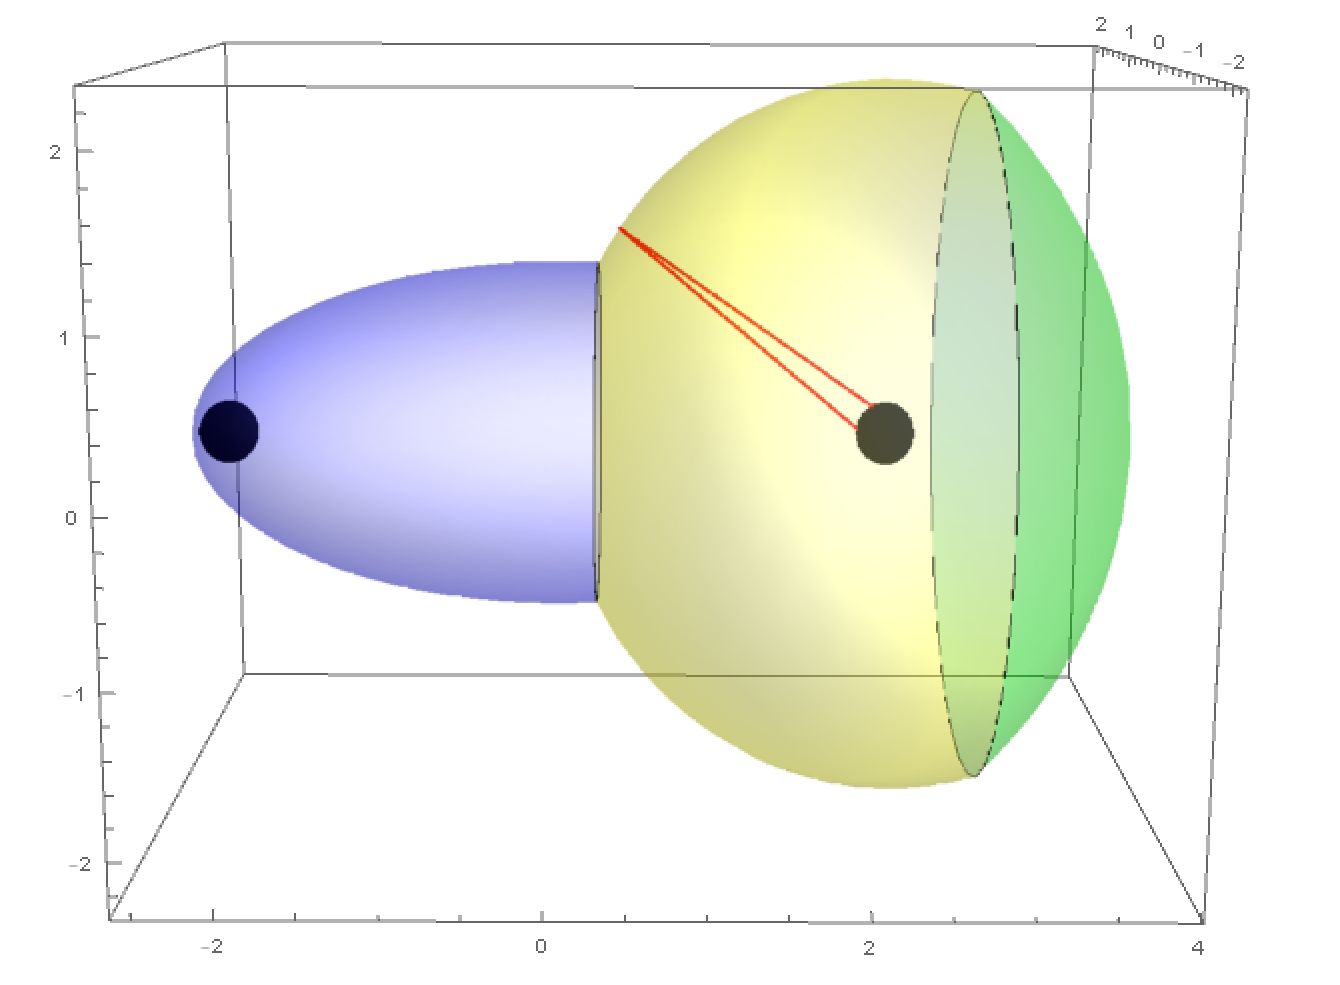
\includegraphics[width=0.6\textwidth]{q2_plot2.png}
        \caption{第二问plot2}\label{fig:第二问plot2}
    \end{figure}

    \begin{figure}[H]
        \centering
        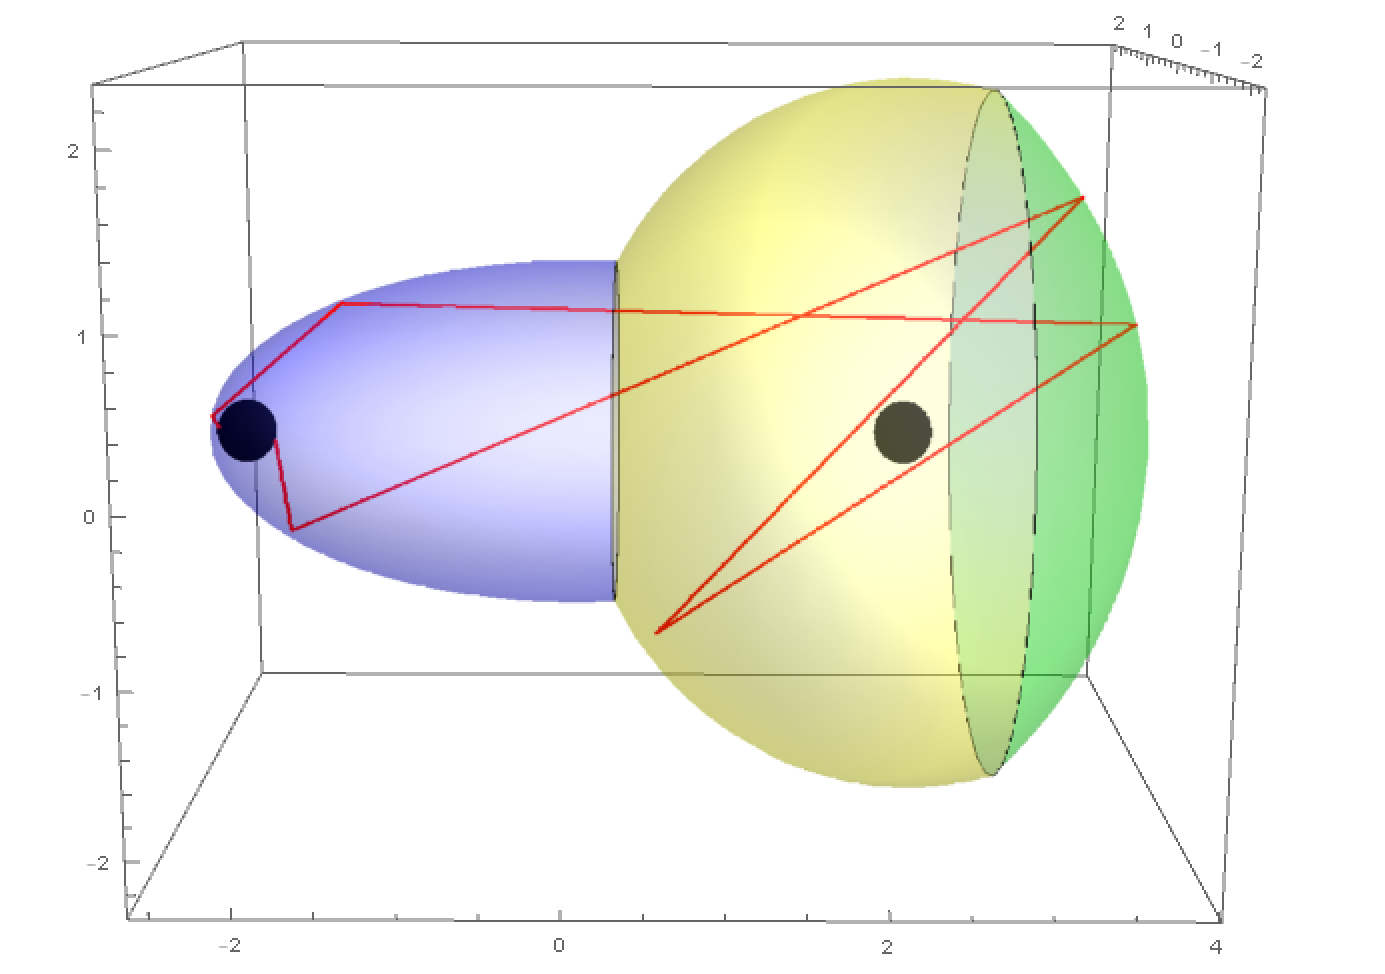
\includegraphics[width=0.6\textwidth]{q2_plot3.png}
        \caption{第二问plot3}\label{fig:第二问plot3}
    \end{figure}

    \begin{figure}[H]
        \centering
        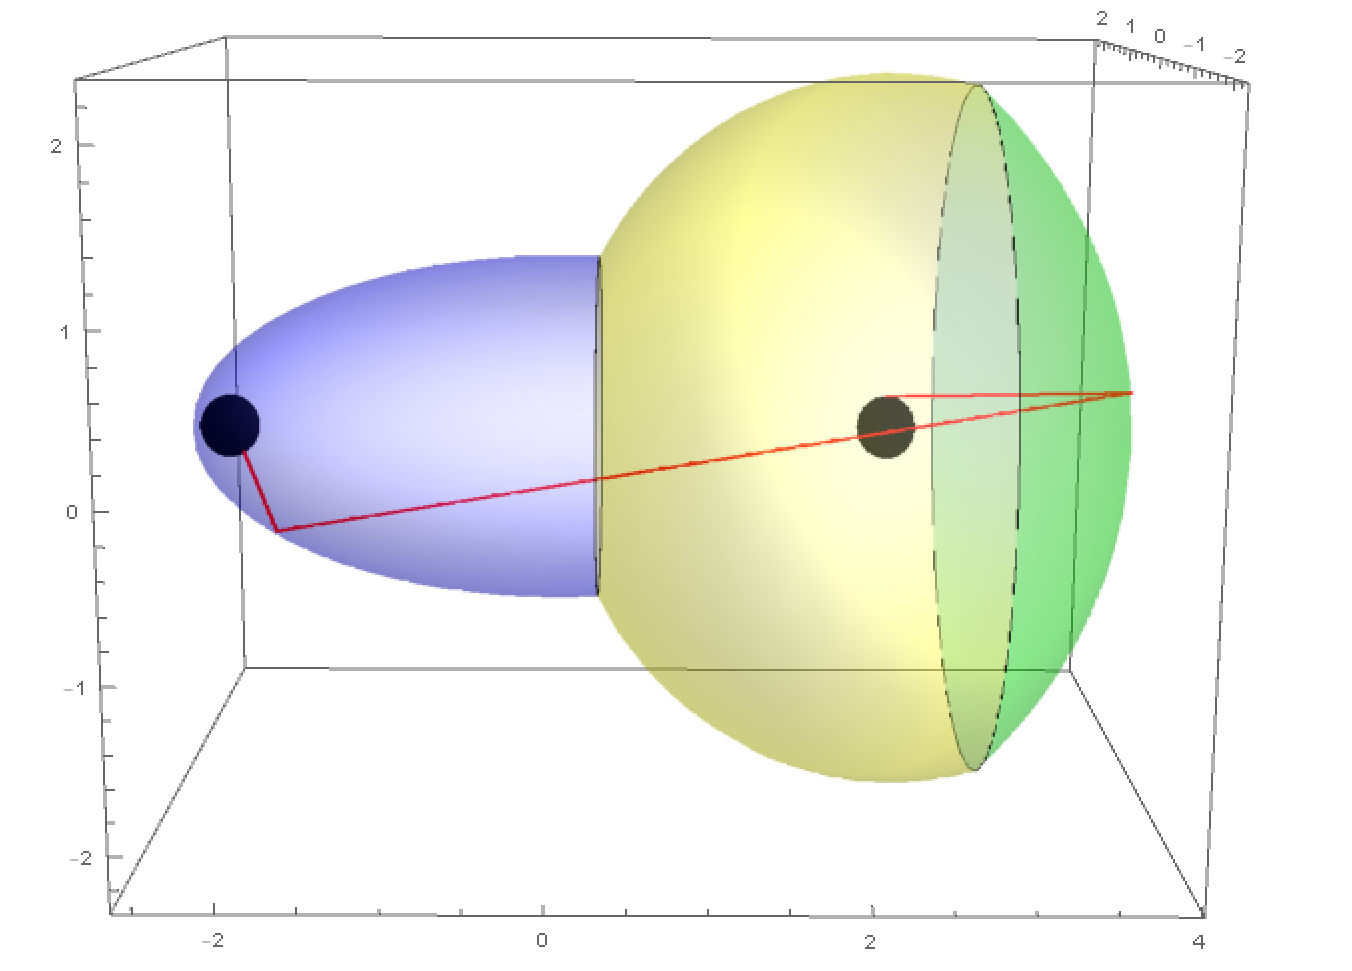
\includegraphics[width=0.6\textwidth]{q2_plot4.png}
        \caption{第二问plot4}\label{fig:第二问plot4}
    \end{figure}

    \begin{figure}[H]
        \centering
        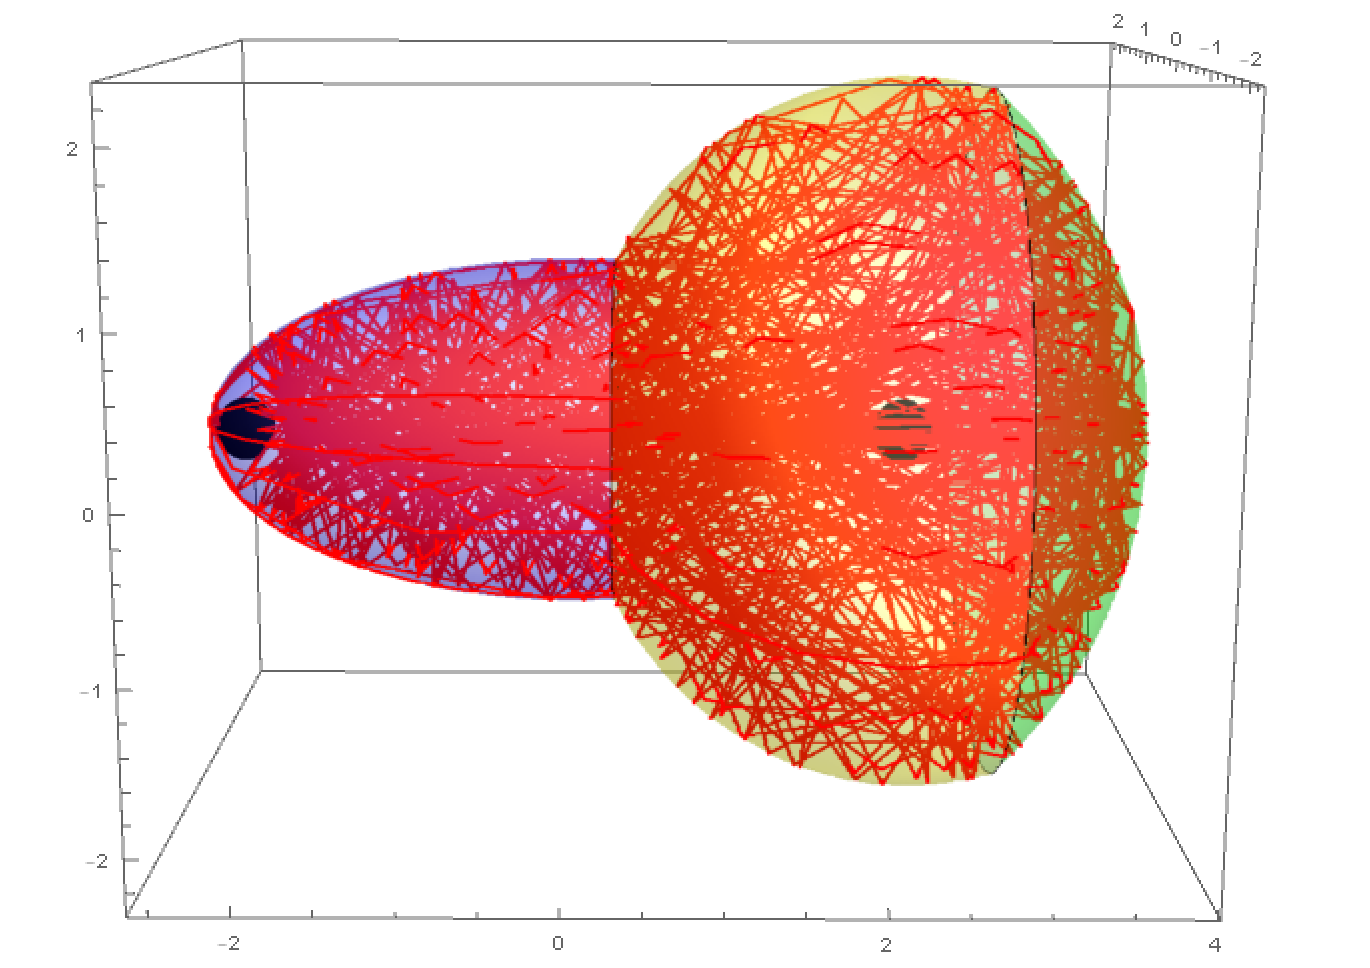
\includegraphics[width=0.6\textwidth]{q2_plot5.png}
        \caption{第二问plot5}\label{fig:第二问plot5}
    \end{figure}

    \begin{figure}[H]
        \centering
        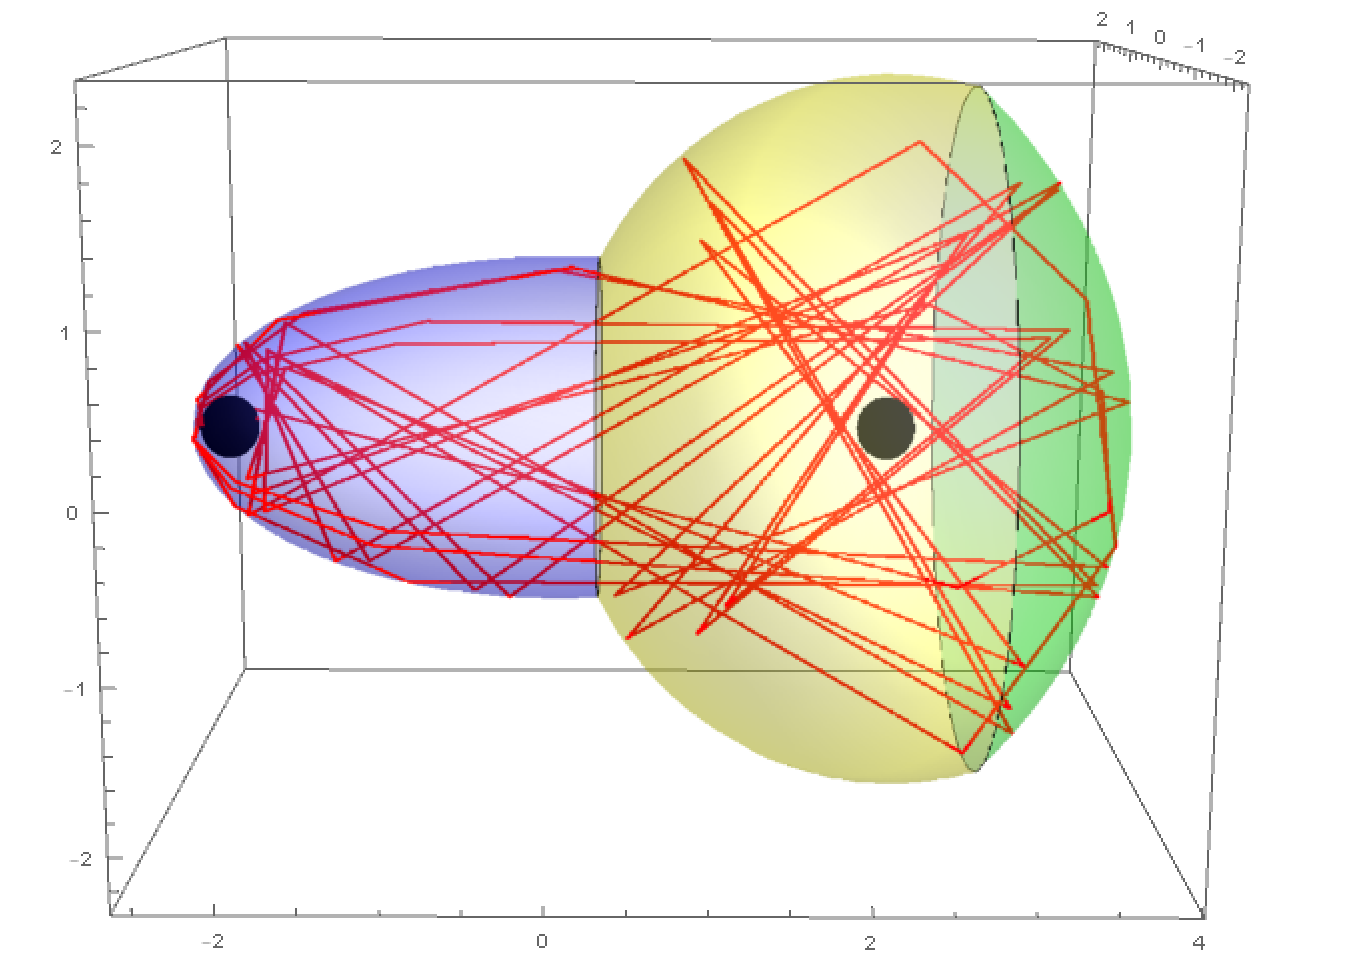
\includegraphics[width=0.6\textwidth]{q2_plot6.png}
        \caption{第二问plot6}\label{fig:第二问plot6}
    \end{figure}

    \subsection{第3-5问}
    
    这几问用的都是code文件夹中"Q3-5.c",需要手动修改参数,共选取了五组RA,RB,输出数据文件为data/experiment文件夹中,可以查看试验的结果。

    因程序运行速度不慢,故试验中取了一个较大的反射次数上限,使得在减小RA,RB的时候,因反射次数太多而被舍弃的光线数都为0。

    五次试验的结果整理如下表,并进行了数据处理,数据处理见"data/data_analysis.xlsx"excel文件sheet“改进前”。

    % Table generated by Excel2LaTeX from sheet 'Sheet1'
    \begin{table}[H]
        \centering
        \caption{试验数据表}
        \begin{tabular}{|c|c|c|c|c|c|c|c|c|c|}\hline
        \multicolumn{10}{|l|}{实验次数N:10000} \\\hline
        RA    & RB    & $p(A\to A)$ & $p(A\to B)$ & $p(B\to A)$ &$ p(B\to B)$ & $\sigma _{p(A\to B)}$ &$ \sigma _{p(B->A)}$ & $T_A/T_B$ & $\sigma_{T_A/T_B} $\\\hline
        0.2   & 0.2   & 0.5888 & 0.4112 & 0.4127 & 0.5873 & 0.0049 & 0.0049 & 1.0009 & 0.0042 \\\hline
        0.1   & 0.2   & 0.1272 & 0.8728 & 0.2169 & 0.7831 & 0.0033 & 0.0041 & 0.9985 & 0.0048 \\\hline
        0.1   & 0.05  & 0.8930 & 0.1070 & 0.4295 & 0.5705 & 0.0031 & 0.0050 & 1.0009 & 0.0078 \\\hline
        0.02  & 0.02  & 0.8353 & 0.1647 & 0.1643 & 0.8357 & 0.0037 & 0.0037 & 0.9994 & 0.0080 \\\hline
        0.005 & 0.005 & 0.5887 & 0.4113 & 0.4140 & 0.5860 & 0.0049 & 0.0049 & 1.0016 & 0.0042 \\\hline
        \end{tabular}%
        \label{tab:试验数据表}%
    \end{table}%
  
    其中数据处理的方法为

    \begin{align*}
        \sigma_{p(A\to B)}&=\frac{\sqrt{Np(A\to B)(1-p(A\to B))}}{N}\\
        \sigma_{p(B\to A)}&=\frac{\sqrt{Np(B\to A)(1-p(B\to A))}}{N}
    \end{align*}

    $T_A,T_B$分别指热平衡时的温度,不考虑反射面吸热,认为反射率100$\%$,热平衡时应有A到B的热流等于B到A的热流,即$P(A\to B)=P(B\to A)$

    其中
    \begin{align*}
        P(A\to B)&=\sigma T_A^4(4\pi R_A^2)p(A\to B)\\
        P(B\to A)&=\sigma T_B^4(4\pi R_B^2)p(B\to A)
    \end{align*}

    $\sigma$为斯特藩-玻尔兹曼常数。于是

    \begin{align*}
        \frac{T_A}{T_B}&=\sqrt{\frac{R_B}{R_A}}(\frac{p(B\to A)}{p(A\to B)})^{1/4}\\
        \sigma_{{T_A}/{T_B}}&=\frac{T_A}{T_B}\sqrt{(\frac{\sigma_{p(B\to A)}}{4p(B\to A)})^2+(\frac{\sigma_{p(A\to B)}}{p(A\to B)})^2}
    \end{align*}

    可以看出,无论RA,RB取何值,$T_A/T_B$与1的差都显著小于其不确定度。可见,这五种情况下A,B达到热平衡时温度都相等,热力学第二定律成立。

    \section{进一步验证———重复实验}

    如果把每一次从A,B分别发射10000条随机光线称为一次试验,每一次试验我们都能得到$T_A/T_B$及其不确定度,我们可以在程序中直接将它算出,而不用向上面那样用excel计算。同时,多次试验表明,存在少数情况,1并不落在不确定度范围之内,这使得多次试验十分有必要。

    code文件夹源代码"Q3-5(improved).c"是实现这一功能的代码,手动设置RA,RB和试验次数,将在data/improved文件夹输出每次试验的$T_A/T_B$及其不确定度。设置实验次数为20次,重新计算3-5问,原始数据见data/improved文件夹。
    
    整理得到下表,数据处理见"data/data_analysis.xlsx"excel文件sheet“改进后”。

    % Table generated by Excel2LaTeX from sheet 'Sheet2'
\begin{table}[H]
    \centering
    \caption{改进的试验数据表}
      \begin{tabular}{|c|c|c|c|c|c|c|c|c|c|c|}\hline
      \multirow{2}[0]{*}{次数} & \multicolumn{2}{|c}{RA=0.2,RB=0.2} & \multicolumn{2}{|c}{RA=0.1,RB=0.2} & \multicolumn{2}{|c}{RA=0.1,RB=0.05} & \multicolumn{2}{|c}{RA=0.02,RB=0.02} & \multicolumn{2}{|c|}{RA=0.005,RB=0.005} \\\cline{2-11}
            & $T_A/T_B$ & $\sigma_{T_A/T_B} $ & $T_A/T_B$ & $\sigma_{T_A/T_B} $& $T_A/T_B$ & $\sigma_{T_A/T_B} $ & $T_A/T_B$ & $\sigma_{T_A/T_B} $ & $T_A/T_B$ & $\sigma_{T_A/T_B} $ \\\hline
      1     & 1.0014 & 0.0043 & 1.0006 & 0.0048 & 0.9988 & 0.0076 & 1.0096 & 0.0081 & 0.9971 & 0.0042 \\\hline
      2     & 0.9960 & 0.0042 & 0.9946 & 0.0049 & 1.0147 & 0.0081 & 0.9974 & 0.0080 & 1.0010 & 0.0043 \\\hline
      3     & 1.0038 & 0.0042 & 1.0030 & 0.0048 & 0.9941 & 0.0076 & 1.0211 & 0.0081 & 0.9985 & 0.0043 \\\hline
      4     & 1.0020 & 0.0043 & 0.9927 & 0.0049 & 0.9884 & 0.0076 & 1.0004 & 0.0080 & 1.0005 & 0.0043 \\\hline
      5     & 1.0016 & 0.0042 & 0.9969 & 0.0049 & 0.9892 & 0.0075 & 0.9998 & 0.0079 & 1.0022 & 0.0043 \\\hline
      6     & 1.0023 & 0.0043 & 1.0008 & 0.0048 & 1.0076 & 0.0079 & 0.9905 & 0.0079 & 1.0082 & 0.0043 \\\hline
      7     & 1.0071 & 0.0043 & 1.0044 & 0.0048 & 1.0061 & 0.0078 & 0.9963 & 0.0079 & 0.9951 & 0.0042 \\\hline
      8     & 0.9979 & 0.0042 & 1.0117 & 0.0047 & 0.9928 & 0.0076 & 0.9963 & 0.0079 & 1.0031 & 0.0043 \\\hline
      9     & 1.0016 & 0.0042 & 0.9954 & 0.0049 & 1.0045 & 0.0078 & 0.9899 & 0.0079 & 0.9945 & 0.0042 \\\hline
      10    & 1.0019 & 0.0043 & 1.0028 & 0.0048 & 0.9986 & 0.0077 & 0.9878 & 0.0079 & 1.0037 & 0.0042 \\\hline
      11    & 0.9944 & 0.0042 & 0.9949 & 0.0049 & 0.9965 & 0.0077 & 1.0031 & 0.0080 & 0.9929 & 0.0043 \\\hline
      12    & 0.9930 & 0.0042 & 1.0003 & 0.0048 & 1.0036 & 0.0078 & 0.9944 & 0.0079 & 1.0004 & 0.0042 \\\hline
      13    & 0.9979 & 0.0042 & 1.0005 & 0.0048 & 1.0016 & 0.0078 & 1.0060 & 0.0080 & 1.0004 & 0.0042 \\\hline
      14    & 1.0013 & 0.0042 & 1.0045 & 0.0048 & 0.9922 & 0.0075 & 1.0061 & 0.0081 & 1.0057 & 0.0042 \\\hline
      15    & 1.0074 & 0.0043 & 0.9950 & 0.0049 & 1.0004 & 0.0078 & 1.0121 & 0.0080 & 0.9973 & 0.0042 \\\hline
      16    & 0.9923 & 0.0042 & 0.9965 & 0.0049 & 1.0025 & 0.0078 & 0.9975 & 0.0081 & 1.0025 & 0.0043 \\\hline
      17    & 1.0037 & 0.0043 & 0.9927 & 0.0049 & 1.0086 & 0.0078 & 0.9936 & 0.0080 & 0.9989 & 0.0042 \\\hline
      18    & 0.9980 & 0.0043 & 0.9991 & 0.0049 & 1.0012 & 0.0078 & 0.9826 & 0.0080 & 0.9945 & 0.0042 \\\hline
      19    & 1.0044 & 0.0042 & 0.9967 & 0.0049 & 1.0012 & 0.0078 & 1.0042 & 0.0080 & 1.0079 & 0.0043 \\\hline
      20    & 1.0023 & 0.0043 & 1.0006 & 0.0048 & 0.9950 & 0.0077 & 0.9928 & 0.0080 & 0.9938 & 0.0042 \\\hline
      \textbf{平均 }   & \textbf{1.0005} & \textbf{0.0009} & \textbf{0.9992 }& \textbf{0.0011 }&\textbf{ 0.9999} &\textbf{ 0.0017} & \textbf{0.9991} &\textbf{ 0.0018} & \textbf{0.9999} &\textbf{ 0.0009 }\\\hline
      \end{tabular}%
    \label{tab:改进的试验数据表}%
  \end{table}%
  
  其中$T_A/T_B$是二十次试验值的算数平均值。由于固定条件下$T_A/T_B$的不确定度都近似相等,近似为一个常数,则平均值的不确定度为这个常数除以$\sqrt{20}$。

  可以看出,各个条件下$T_A/T_B$测量值分立1的两侧,而1都落在测量值的不确定度范围之内。进而说明,随着RA,RB的减小,A,B温度相等,热力学第二定律成立。

\end{document}